\section{Apendice 1. Ejemplo de utilización del plugin SERIALIZARDWG.}

\begin{figure}[h]
\begin{center}
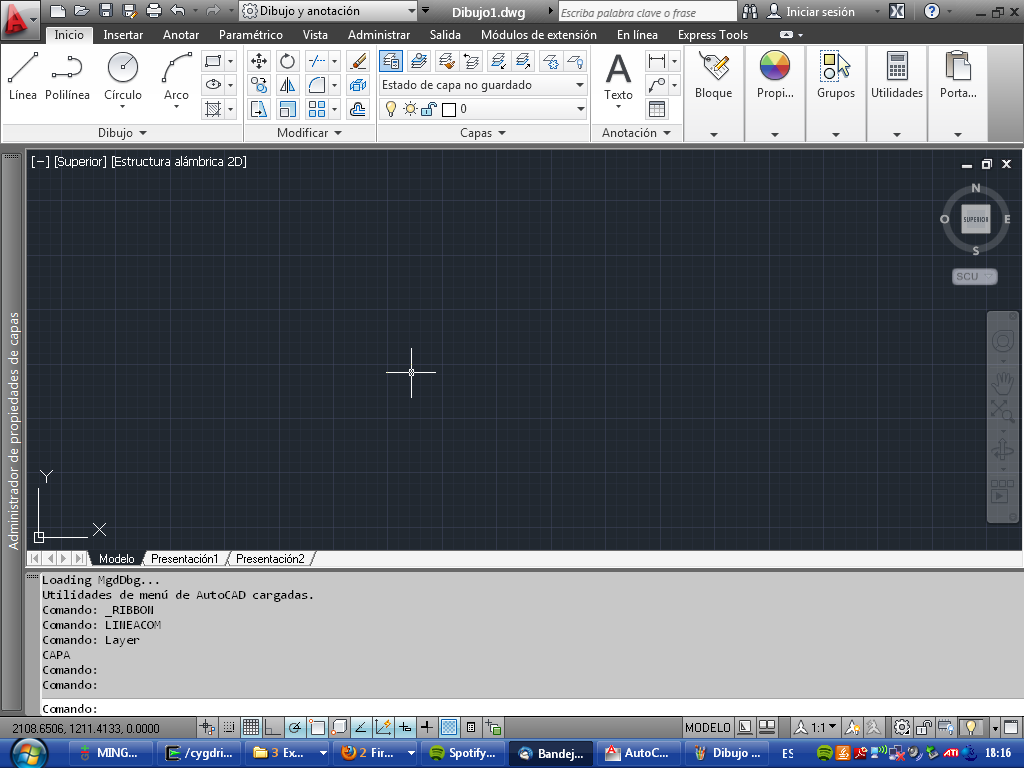
\includegraphics[width=\textwidth]{imgs/autocad0}
\caption{Aplicación AutoCAD.}
\end{center}
\end{figure}


\begin{figure}[h]
\begin{center}
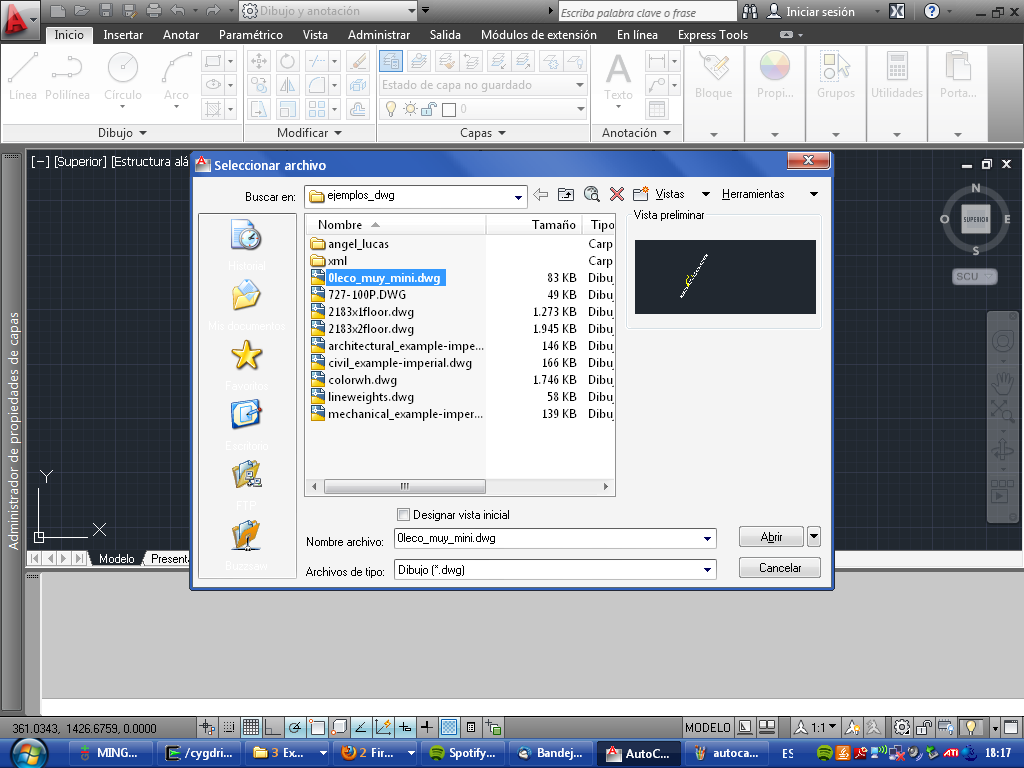
\includegraphics[width=\textwidth]{imgs/autocad1}
\caption{Aplicación AutoCAD abriendo fichero DWG.}
\end{center}
\end{figure}

\begin{figure}[h]
\begin{center}
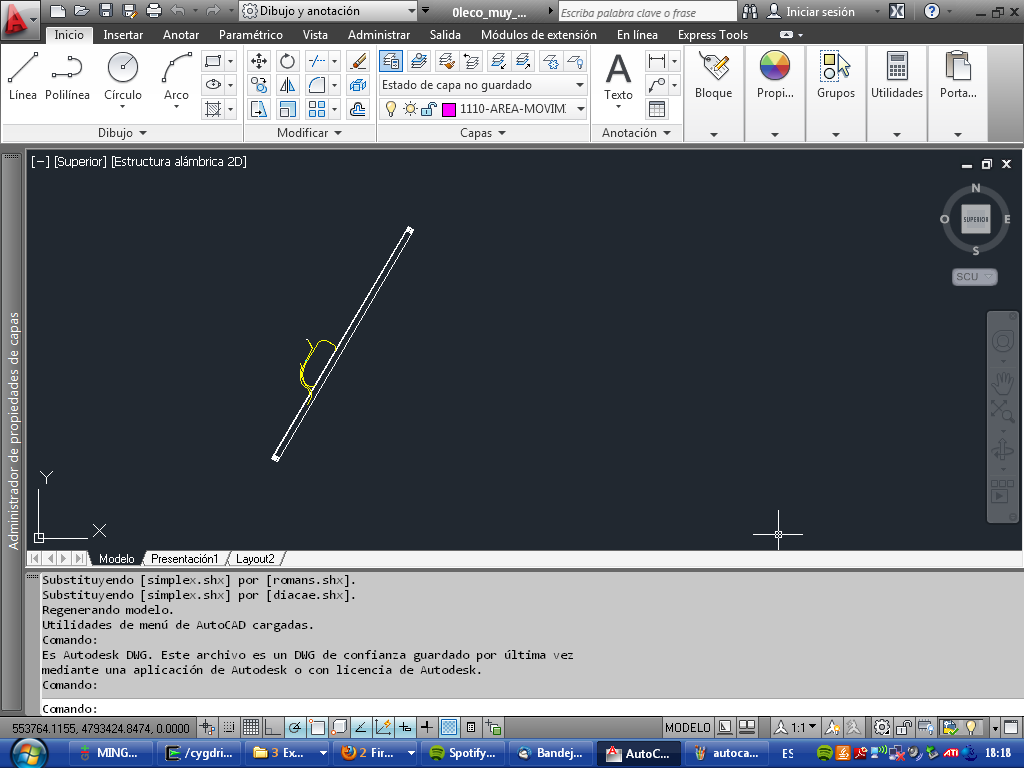
\includegraphics[width=\textwidth]{imgs/autocad2}
\caption{Aplicación AutoCAD mostrando fichero DWG.}
\end{center}
\end{figure}

\begin{figure}[h]
\begin{center}
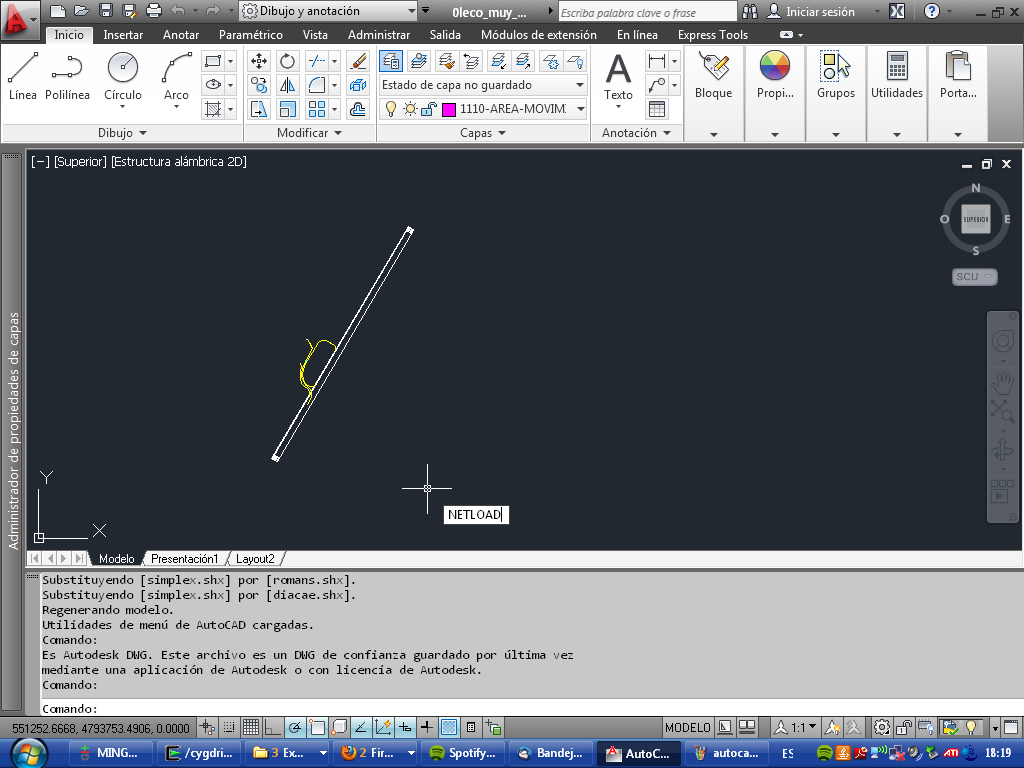
\includegraphics[width=\textwidth]{imgs/autocad3}
\caption{Invocacion del comando NETLOAD para cargar el plugin.}
\end{center}
\end{figure}

\begin{figure}[h]
\begin{center}
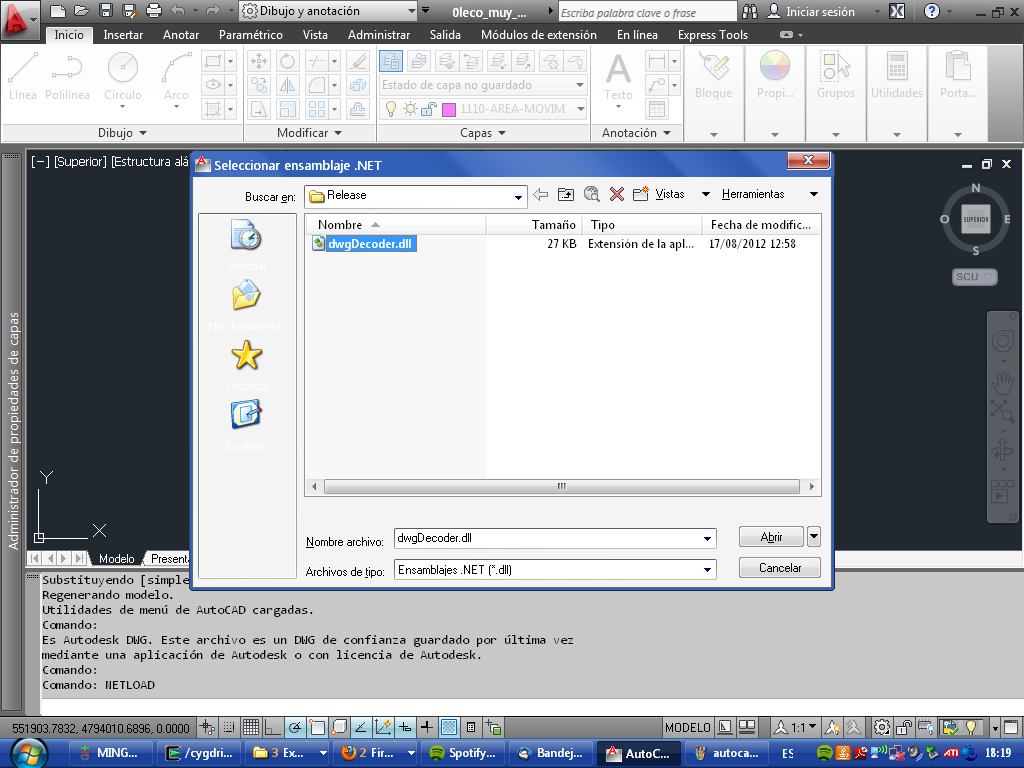
\includegraphics[width=\textwidth]{imgs/autocad4}
\caption{Selección del fichero DLL que cotiene el plugin.}
\end{center}
\end{figure}

\begin{figure}[h]
\begin{center}
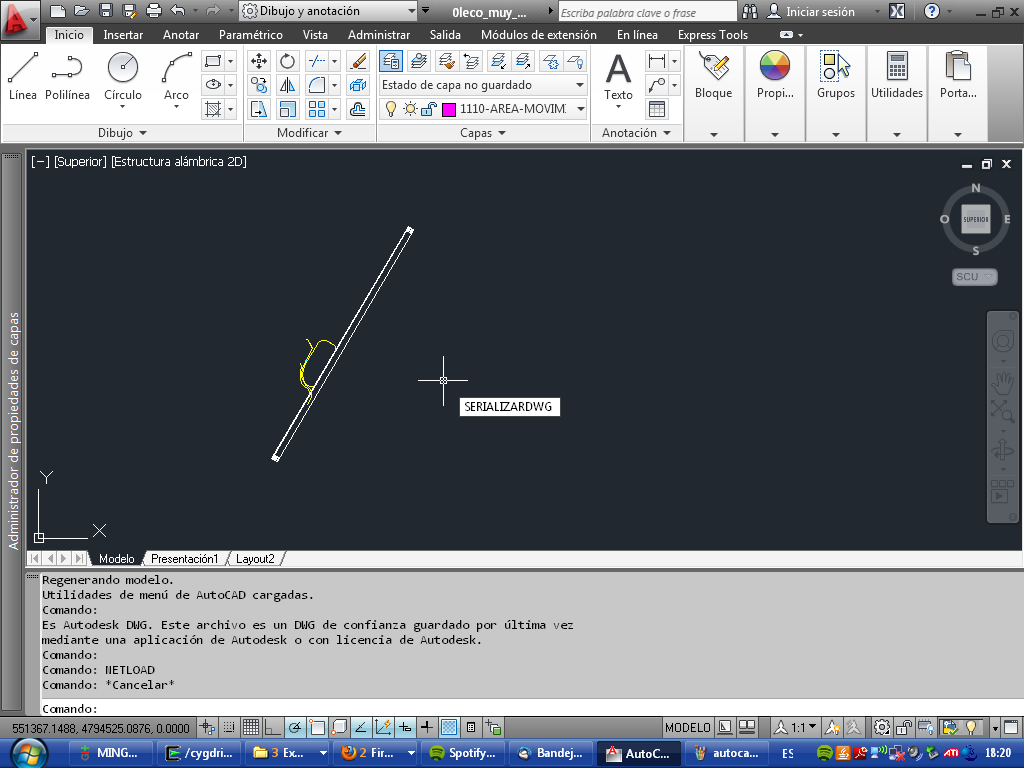
\includegraphics[width=\textwidth]{imgs/autocad5}
\caption{Invocación del comando SERIALIZARDWG implementado en el plugin.}
\end{center}
\end{figure}

\begin{figure}[h]
\begin{center}
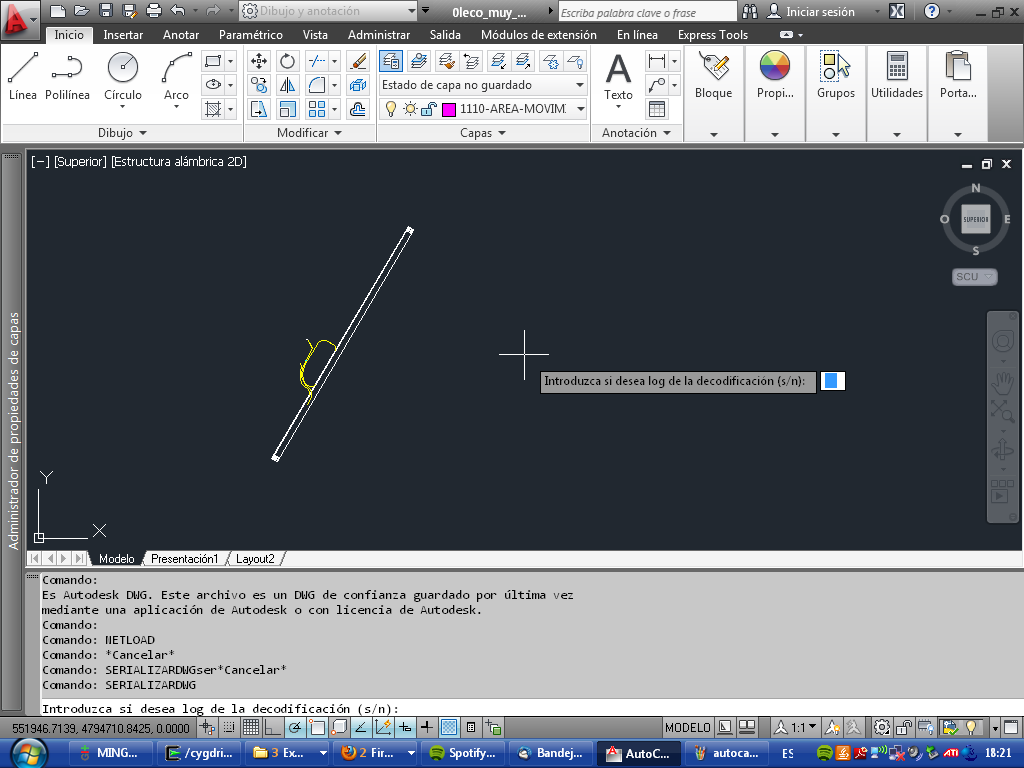
\includegraphics[width=\textwidth]{imgs/autocad6}
\caption{Usuario configurando si desea log del proceso de extracción.}
\end{center}
\end{figure}

\begin{figure}[h]
\begin{center}
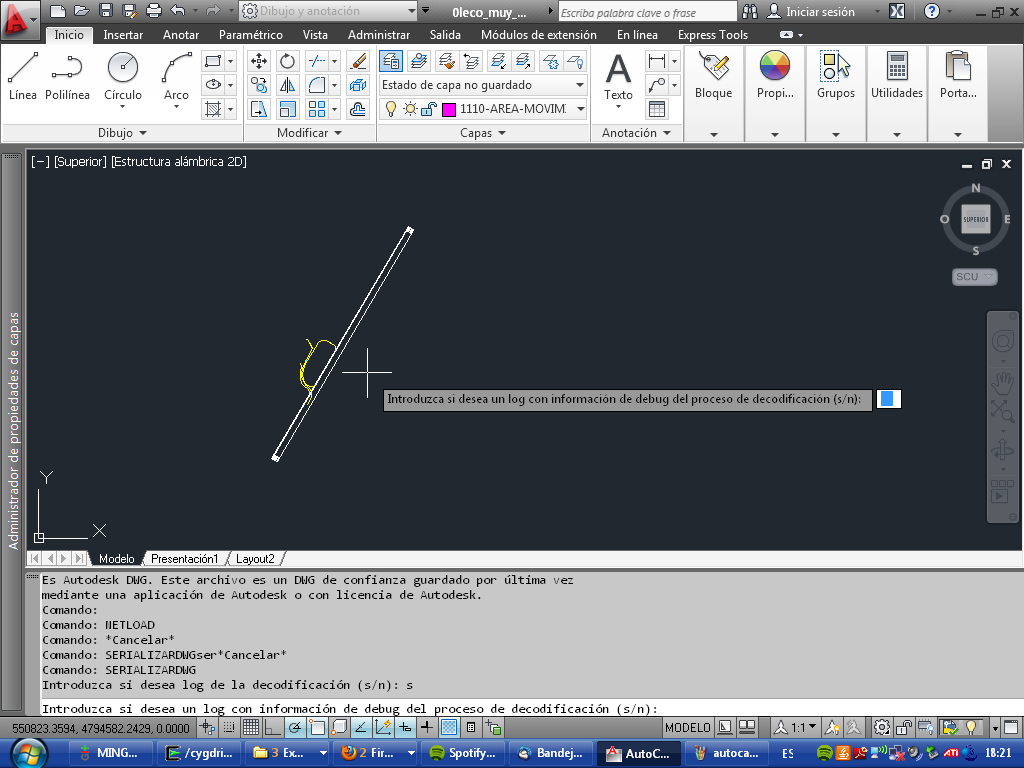
\includegraphics[width=\textwidth]{imgs/autocad7}
\caption{Usuario configurando si desea incorporar información de debug al log del proceso de extracción.}
\end{center}
\end{figure}

\begin{figure}[h]
\begin{center}
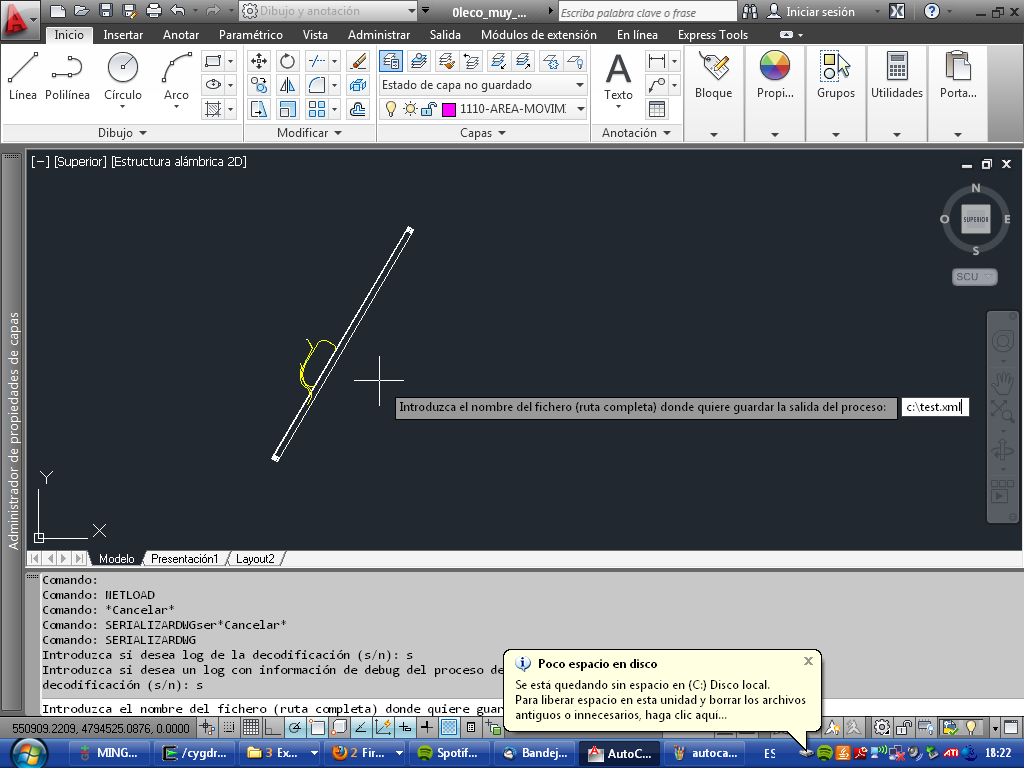
\includegraphics[width=\textwidth]{imgs/autocad8}
\caption{Usuario configurando la ruta donde se almacenará el fichero con la salida del proceso de extracción.}
\end{center}
\end{figure}

\begin{figure}[h]
\begin{center}
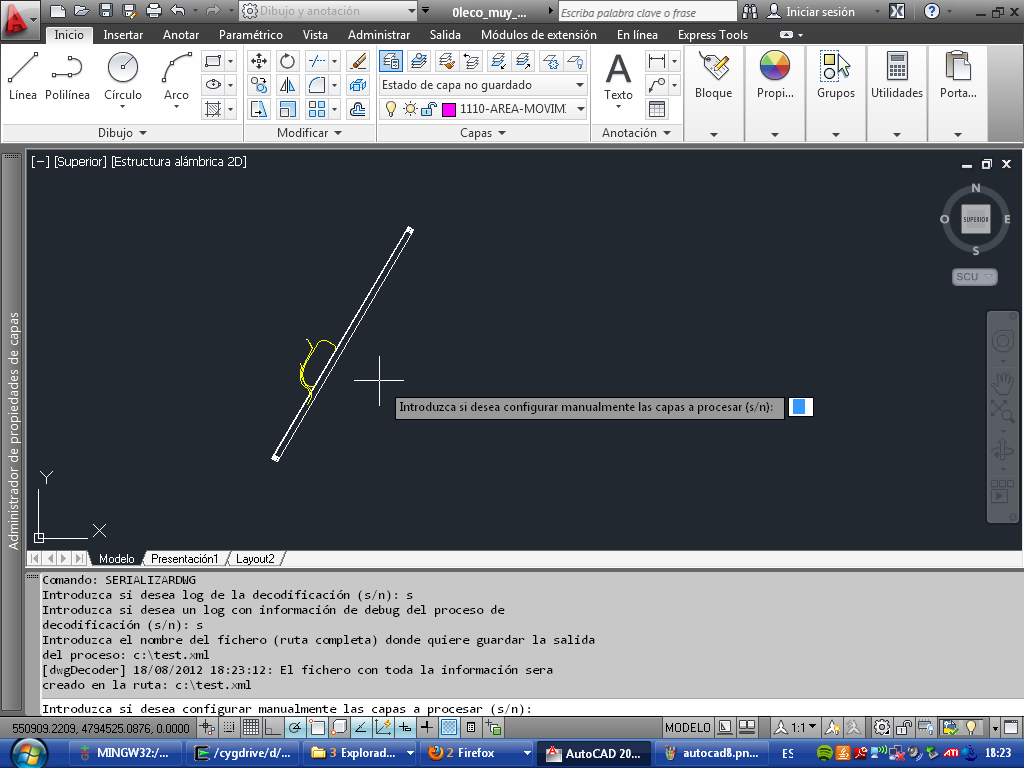
\includegraphics[width=\textwidth]{imgs/autocad9}
\caption{Usuario configurando si desea seleccionar las capas que deben ser procesadas.}
\end{center}
\end{figure}

\begin{figure}[h]
\begin{center}
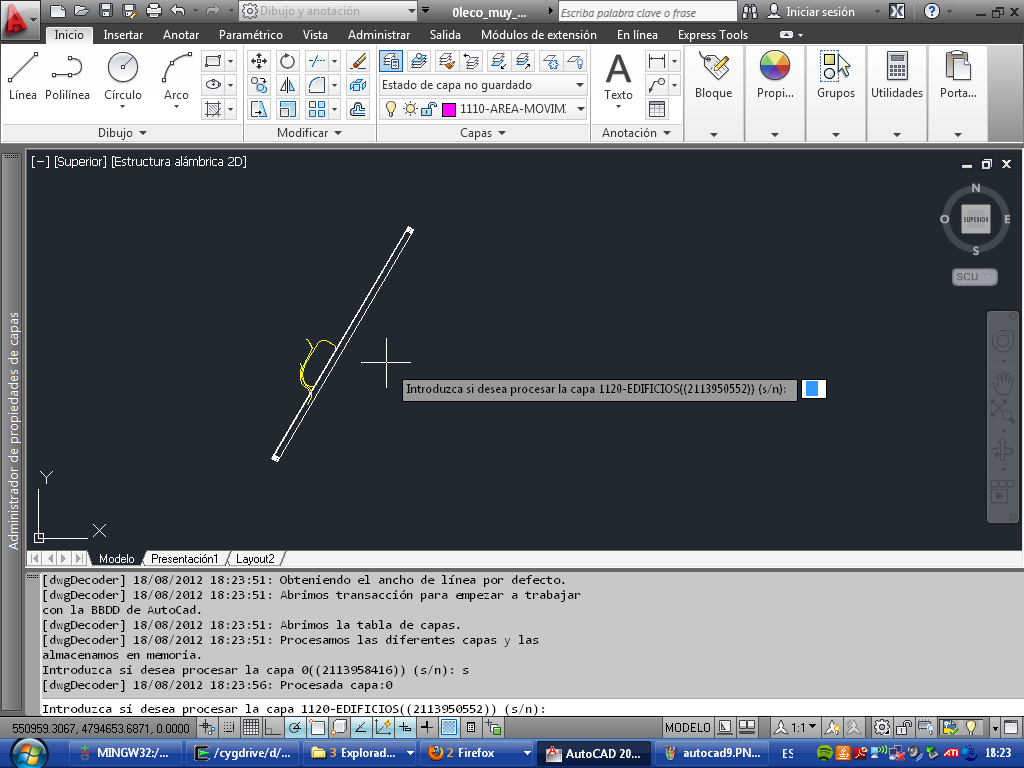
\includegraphics[width=\textwidth]{imgs/autocad10}
\caption{Usuario configurando si desea incluir una capa en el proceso.}
\end{center}
\end{figure}

\begin{figure}[h]
\begin{center}
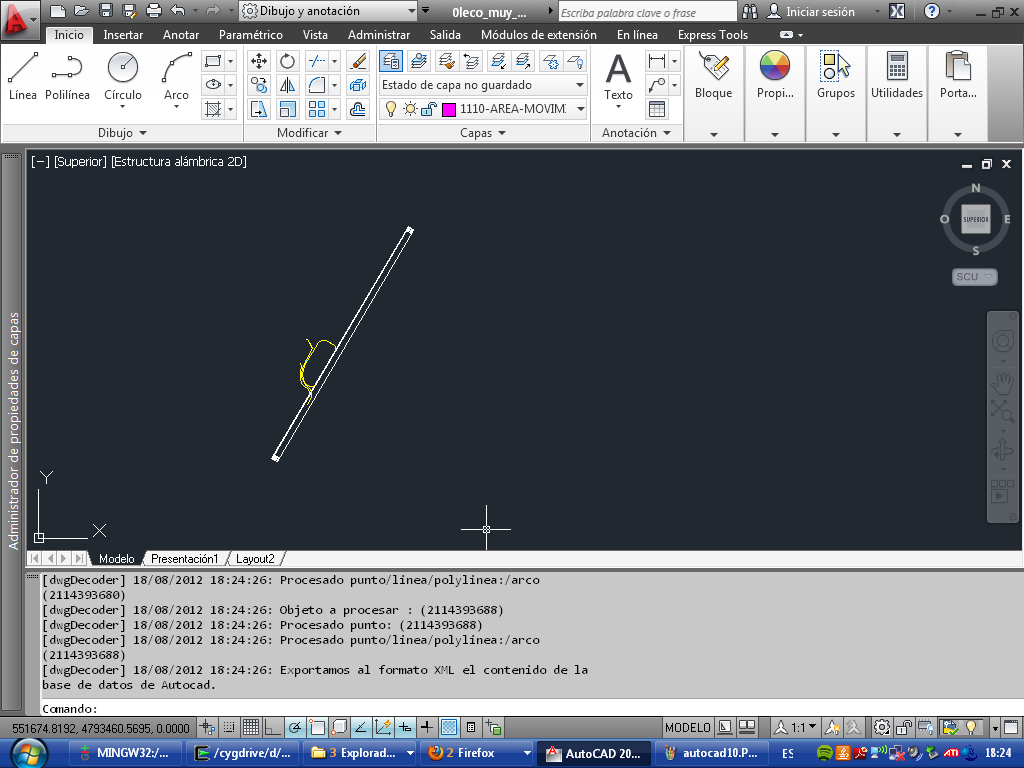
\includegraphics[width=\textwidth]{imgs/autocad11}
\caption{Aplicación AutoCad indicando que la exportación ha finalizado correctamente.}
\end{center}
\end{figure}


